\documentclass[11pt]{article}
\input{/Users/markwang/.preamble}
\begin{document}


\section*{Inferences in Regression and Correlation Analysis}


\subsection*{2.1 Inference Concerning $\beta_1$}


\begin{defn*}
    \textbf{Inference concerning $\beta_1$} Test concerning $\beta_1$ is of the form 
    \[
        \begin{cases*}
            \mathcal{H}_0: \beta_1 = 0\\
            \mathcal{H}_{\alpha}: \beta_1 \neq 0  
        \end{cases*}
    \]
    $\beta_1 = 0$ implies that there is no linear association between $Y$ and $X$. On assumption of gaussian noise, there is also no relation of any type between $Y$ and $X$, since probability of $Y$ are identical for all levels of $X$ 
\end{defn*} 


\begin{defn*}
    \textbf{Linear estimators} Least square estimator $\hat{\beta}_1$ is a linear estimator
    \[
        \hat{\beta}_1 = \sum_i k_i y_i \quad \quad k_i = \frac{x_i -\overline{x}}{\sum_j (x_j - \overline{x})^2}
    \]
    with properties
    \[
        \sum k_i = 0 \quad \sum k_i x_i = 1 \quad \sum k_i^2 = \frac{1}{S_{XX}}
    \]
    \begin{proof}
        Note
        \[
            \sum (x_i - \overline{x})(y_i - \overline{y}) = \sum (x_i - \overline{x})y_i - \sum (x_i - \overline{x})\overline{y} = \sum (x_i - \overline{x})y_i \quad \text{by $\sum (x_i - \overline{x}) = 0$}
        \]
        the result follows. Proof of properties are simple, i.e.
        \[
            \sum k_i = \sum_i \left( \frac{x_i - \overline{x}}{\sum_j (x_j - \overline{x})^2} \right) = \frac{1}{\sum_j (x_j - \overline{x})^2} \sum_i (x_i - \overline{x}) = 0
        \]
    \end{proof}
\end{defn*}

\begin{defn*}
    \textbf{Sampling distribution of $\hat{\beta}_1$} The sampling distribution of $\hat{\beta}_1$ refers to different values of the estimator obtained with repeated sampling when the levels of the predictor variable $X$ are held constant from sample to sample. Given $\hat{\beta}_1$ 
    \[
        \hat{\beta}_1 = \frac{\sum (x_i - \overline{x})(y_i - \overline{y})}{\sum (x_i - \overline{x})^2}
    \]
    The sampling distribution of $\hat{\beta}_1$ is \textbf{normal} with mean and variance,
    \[
        \E(\hat{\beta}_1 | X) = \beta_1 \quad Var(\hat{\beta}_1 | X) = \frac{\sigma^2}{\sum (x_i - \overline{x})^2} = \frac{\sigma^2}{S_{XX}}
    \]
    \[
        \hat{\beta}_1 \sim \norm(\beta_1, \frac{\sigma^2}{S_{XX}})
    \]
    \begin{proof}
        $ $\\
        \begin{enumerate}
            \item \textbf{Mean and variance}
            \[
                \E(\hat{\beta}_1) = \E\{ \sum k_i y_i \} \overset{ind}{=} \sum (k_i \E\{y_i \}) = \sum k_i(\beta_0 + \beta_1 x_i) = \beta_0 \sum k_i + \beta_1 \sum k_i x_i = \beta_1
            \]
            \[
                Var(\hat{\beta}_1) = Var\left( \sum k_i y_i \right) = \sum k_i^2 Var(y_i) = \sum k_i^2\sigma^2 = \sigma^2 \sum k_i^2 = \frac{\sigma^2}{S_{XX}}
            \]
            with last step of both derivation given by properties of $\hat{\beta}_1$ as a linear estimator. 
            \item \textbf{Normality} of sampling distribution given by the fact that $\hat{\beta}_1$ is a linear combination of $y_i$s. Since $y_i \overset{i.i.d}{\sim} \norm(\beta_0 + \beta1 x_i , \sigma^2)$, the estimator is normaly distributed because it is a linear combination of independent normal random variables
            \item \textbf{Estimated variance} We can estimate the variance of $\hat{\beta}_1$ by substituting $\sigma^2$ (unknown) with its unbiased estimator MSE $s^2$
            \[
                s^2 (\hat{\beta}_1) = \frac{MSE}{S_{XX}} \quad \text{ where } \quad MSE = \frac{\sum e_i^2}{n-2}
            \]
            Note $s^2$ carries a denominator of $S_{XX}$, this is from the variance of $\hat{\beta}_1$, we are simply substituting the unknown $\sigma^2$ with $MSE$
        \end{enumerate}
    \end{proof}
\end{defn*}


\begin{defn*}
    \textbf{standardization of $\hat{\beta}_1$} \\
    Standardization of sampling distribution of $\hat{\beta}_1$ gives 
    \[
        Z =  \frac{\hat{\beta}_1 - \beta_1}{\sigma(\hat{\beta}_1)} = \norm(0, 1) \quad \text{ wher } \quad \sigma(\hat{\beta}_1) = \frac{\sigma}{\sqrt{S_{XX}}}
    \]
    Usually, have to estimate standard error $\sigma(\hat{\beta}_1)$ with $s(\hat{\beta}_1)$. Standardization where the denominator is an estimated standard error is called \textbf{studentized statistic}, given by
    \[
        T = \frac{\hat{\beta}_1 - \beta_1}{s(\hat{\beta}_1)} \sim t_{n-2} \quad  \text{ where } \quad s^2(\hat{\beta}_1) = \frac{MSE}{S_{XX}}
    \]
    \begin{proof}
        Assume proposition 
        \[
            \frac{\sum (\hat{e}_i)^2 }{\sigma^2} \sim \chi^2_{n-2}
        \]
        Then we have 
        \[
            \frac{\hat{\beta}_1 - \beta_1}{s(\hat{\beta}_1)} 
            = \frac{\hat{\beta}_1 - \beta_1}{\sigma(\hat{\beta}_1)} \Biggm/ \frac{s(\hat{\beta}_1)}{\sigma(\hat{\beta}_1)} 
            = \frac{\hat{\beta}_1 - \beta_1}{\sigma(\hat{\beta}_1)} \Biggm/ \sqrt{\frac{\sum e_i^2 S_{XX}}{(n-2) S_{XX} \sigma^2 }}
            \sim \frac{Z}{\sqrt{\chi^2_{n-2} \Big/ (n-2)}} 
            = t_{n-2}
        \]
    \end{proof}
\end{defn*}


\begin{defn*}
    \textbf{Confidence Interval and test for $\beta_1$} \\
    We use the previously derived distribution as a pivot
    \[
        \Pr\left(t_{\alpha/2, n-2} \leq \frac{\hat{\beta}_1 - \beta_1}{s(\hat{\beta}_1)} \leq t_{1-\alpha/2, n-2}\right) = 1-\alpha
    \]
    \[
        \Pr\left(\hat{\beta}_1 - s(\hat{\beta}_1)t_{1-\alpha/2, n-2} \leq \beta_1 \leq \hat{\beta}_1 + s(\hat{\beta}_1)t_{1-\alpha/2, n-2} \right) = 1-\alpha
    \]
    Hence the confidence interval is given by 
    \[
        \hat{\beta}_1 \pm s(\hat{\beta}_1)t_{1-\alpha/2, n-2} \quad \text{ where }\quad s^2(\hat{\beta}_1) = \frac{MSE}{S_{XX}}
    \]
    For 2-sided tests
    \[
        \begin{cases*}
            \mathcal{H}_0: \beta_1 = b\\
            \mathcal{H}_{\alpha}: \beta_1 \neq b\\  
        \end{cases*}
    \]
    We compute test statistics 
    \[
        t^* = \frac{\hat{\beta}_1 - b}{s(\hat{\beta}_1)} \quad \text{ and reject $\mathcal{H}_0$ if }  |t^*| > t_{1-\alpha/2, n-2}
    \]
\end{defn*}


\subsection*{2.2 Inference Concerning of $\hat{\beta}_0$}

\begin{defn*}
    \textbf{Sampling Distribution of $\hat{\beta}_0$} \\
    Given point estimator 
    \[
        \hat{\beta}_0 = \overline{y} - \beta_1 \overline{x}
    \]
    $\hat{\beta}_0$ refers to different values of $\beta_0$ that would be obtained with repeated sampling when levels of predictor variable $x$ are held constant from sample to sample. The \textbf{sampling distribution of $\hat{\beta}_0$} is \textbf{normal} with mean and variance
    \[
        \E(\hat{\beta}_0) = \beta_0 \quad \quad Var(\hat{\beta}_0) = \sigma^2 \left[ \frac{1}{n} + \frac{\overline{x}^2}{\sum (x_i - \overline{x})^2} \right] = \sigma^2 \left[ \frac{1}{n} + \frac{\overline{x}^2}{S_{XX}} \right]
    \]
    \begin{proof}
        The normality follows because $\hat{\beta}_0$ is also a linear estimator of $y_i$s. We can estimate $Var(\hat{\beta}_0)$ by replacing $\sigma^2$ with MSE, as before
        \[
            s^2(\hat{\beta}_0) = MSE \left[ \frac{1}{n} + \frac{\overline{x}^2}{S_{XX}} \right]
        \] 
    \end{proof}
\end{defn*}

\begin{defn*}
    \textbf{Standardization of $\hat{\beta}_0$} \\
    
    \[
        Z = \frac{\hat{\beta}_0 - \beta_0}{\sigma(\hat{\beta}_0)} \sim t_{n-2} \quad \text{ where }\quad \sigma^2(\hat{\beta}_0) =  \sigma^2 \left[ \frac{1}{n} + \frac{\overline{x}^2}{S_{XX}} \right]
    \]
    \[
        T = \frac{\hat{\beta}_0 - \beta_0}{s(\hat{\beta}_0)} \sim t_{n-2} \quad \text{ where } \quad s^2(\hat{\beta}_0) = MSE \left[ \frac{1}{n} + \frac{\overline{x}^2}{S_{XX}} \right]
    \]
\end{defn*}

\begin{defn*}
    \textbf{Confidence Interval for $\hat{\beta}_0$}\\
    \[
        \hat{\beta}_0 \pm s(\hat{\beta}_0) t_{1-\alpha/2, n-2} \quad \text{ where } \quad s(\hat{\beta}_0) = \sqrt{\frac{\sum e_i^2}{n-2}} \sqrt{\frac{1}{n} + \frac{\overline{x}^2}{S_{XX}}}
    \]
\end{defn*}



\begin{defn*}
    \textbf{Consideration about inference}
    \begin{enumerate}
        \item \textbf{Spacing of $x$ levels} Looking at variance of $\hat{\beta}_0$ and $\hat{\beta}_1$, the larger the spread in $x$ levels, the larger $S_{XX}$ and smaller the variance. 
    \end{enumerate}
\end{defn*}



\subsection*{2.4 Interval Estimation of $\E(Y | X = x^*)$, the population regression line}


\begin{defn*}
    \textbf{Mean estimation} Often times want to estimate mean for one or more probability distribution of $Y$. (i.e. mean $Y$ for low and high $X$ levels). Let $x^*$ be level of $X$ for which we want to estimate the mean response $\hat{y}^*$. The mean response is given by 
    \[
        \E(Y | X = x^*) = E(y^*) = \beta_0 + \beta_1 x^*
    \]
    The idea is that the expectation is a random variable because of the estimated correlation coefficients. We would want to do inference on the mean response. We have a point estimator of the the mean response
    \[
        \hat{y}^* = \hat{\beta}_0 + \hat{\beta}_1 x^*
    \]
    which is simply the estimated response from estimated correlation coefficients and regression function. Note $X = x^*$ is a known constant 
\end{defn*}


\begin{defn*}
    \textbf{Sampling Distribution of mean response estimator $\hat{y}^*$} \\
    The sampling distribution of $\hat{y}^*$ is \textbf{normal} with mean and variance 
    \[
        \E(\hat{y}^*) = \E(\hat{y}|X=x^*) = \beta_0 + \beta_1 x^* \quad \text{($= \E(y^*)$ so unbiased)}
    \]
    \[
        Var(\hat{y}^*) = Var(\hat{y}|X=x^*) = \sigma^2 \left[ \frac{1}{n} + \frac{(x^* - \overline{x})^2}{\sum (x_i - \overline{x})^2} \right] = \sigma^2 \left[ \frac{1}{n} + \frac{(x^* - \overline{x})^2}{S_{XX}} \right]
    \]
    \[
        \hat{y}^* = (\hat{y}|X=x^*) \sim \norm(\beta_0 + \beta_1 x^*, \sigma^2 \left[ \frac{1}{n} + \frac{(x^* - \overline{x})^2}{S_{XX}} \right])
    \]
    Note when $x^*=0$, $Var(\hat{y}^*)$ reduces to variance of $\hat{\beta}_0$. 
    \begin{proof}
        3 parts
        \begin{enumerate}
            \item \textbf{Normality} of $\hat{y}^*$ follows from the fact that it is composed of $\hat{\beta}_0$ and $\hat{\beta}_1$, both of which are linear estimators of $y_i$
            \item \textbf{Mean}
            \[
                \E(\hat{y}^*)=  \E\left( \hat{\beta}_0 + \hat{\beta}_1 x^* \right) = \E(\hat{\beta}_0) + x^* \E(\hat{\beta}_1) = \beta_0 + \beta_1 x^* = \E(y^*)
            \]
            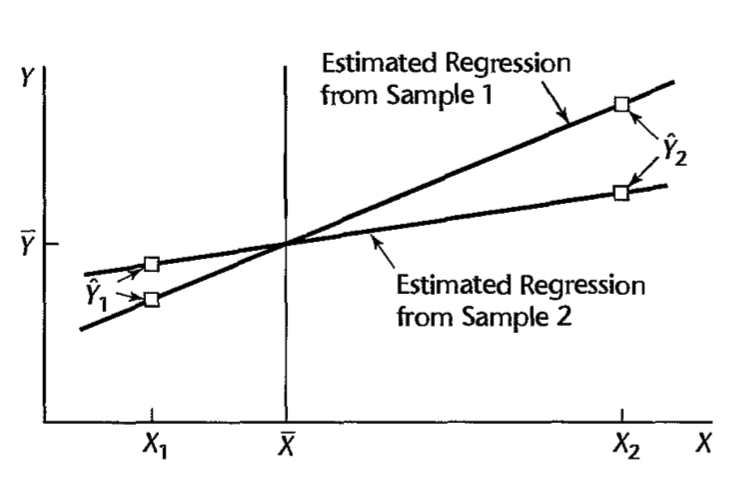
\includegraphics[width=\textwidth/2]{mean_response_var_plot}
            \item \textbf{Variance} Idea is variability of $\hat{y}^*$ is affected by how far $x^*$ is from $\overline{x}$, via 
            \[
                (x^* - \overline{x})^2 = S_{XX}
            \]
            The further $x^*$ is from $\overline{x}$, the greater the variability. Note in plot, $x_1$ near $\overline{x}$, the fitted value $\hat{y}_1$ for two sample regression line (from 2 experiments) are close to each other; the fitted values $\hat{y}_2$ differ substantially due to the fact that $x_2$ is far from $\overline{x}$. In summary, 
            \begin{center}
                \textbf{variation in $\hat{y}^*$ value from sample to sample will be greater when $x^*$ is far from mean than when $x^*$ is near mean} 
            \end{center}
            We can substitute MSE for $\sigma^2$ to obtain $s^2(\hat{y}^*)$. The estimated variance is given by
            \[
                 s^2(\hat{y}^*) = MSE \left[ \frac{1}{n} + \frac{(x^* - \overline{x})^2}{S_{XX}} \right]
            \]
        \end{enumerate}
    \end{proof}
\end{defn*}

\begin{defn*}
    \textbf{Standardization of mean response estimator $\hat{y}^*$}\\
    \[
        Z = \frac{\hat{y}^* - (\beta_0 + \beta_1 x^*)}{\sigma(\hat{y}^*)} \sim \norm(0,1)
    \]
    note $\E(y^*) = \beta_0 + \beta_1 x^*$
    \[
        T = \frac{\hat{y}^* - (\beta_0 + \beta_1 x^*)}{s(\hat{y}^*)} \sim t_{n-2}
    \]
\end{defn*}

\begin{defn*}
    \textbf{Confidence Interval for $\hat{y}^*$}\\
    The $100(1-\alpha)\%$ confidence interval for $\E(Y|X=x^*)=\beta_0 + \beta_1 x^*$ is given by
    \[
        \hat{y}^* \pm s(\hat{y}^*) t_{1-\alpha/2, n-2} = (\hat{\beta}_0 + \hat{\beta}_1 x^*) \pm t_{1-\alpha/2, n-2} \sqrt{\frac{\sum e_i^2}{n-2}}\sqrt{ \frac{1}{n} + \frac{(x^* - \overline{x})^2}{S_{XX}} }
    \]
\end{defn*}


\begin{defn*}
    \textbf{Obervations}
    \begin{enumerate}
        \item variance of $\hat{y}^*$ is smallest when $x^* = \overline{x}$. So in an experiment to estimate mean response at a particular level $x^*$ of predictor variable, the \textbf{precision of the estimate is greatest} if (everything else remain equal) the observations on $X$ are spaced so that $\overline{x} = x^*$
        \item confidence interval for $\hat{y}^*$ not sensitive to moderate departures from assumption of error being normally distributed. The robustness in estimating mean response is related to robustness of Confidence interval for $\beta_0$ and $\beta_1$
    \end{enumerate}
\end{defn*}


\subsection*{2.5 Prediction of New Observations}

\begin{defn*} \textbf{Prediction of New Observations}
    \begin{enumerate}
        \item \textbf{Motivation}  Idea is that we have a model set up given a set of data, and we would want to extrapolate to new data points. The new observation $Y$ is viewed as the result of a new trial, independent of trials on which the regression analysis is based. Let level of $X$ be $x^*$ and the new observation $y^*_{new}$ (which is unknown, and which we want to characterize), assuming that the underlying regression model is still appliacble for basic sample data 
        \item \textbf{Estimate of mean response $\E(y^*)$ vs. Prediction of new response $y^*_{new}$ } \\
        In the former case, we estimate \textbf{mean of distribution of $Y$}. In latter case, we predict an \textbf{individual outcome} drown from the distribution of $Y$. Idea is we have to take into account of the fact that the majority of individual outcomes deviate from the mean response
    \end{enumerate}
\end{defn*}


\begin{defn*}
    \textbf{Prediction Interval for $y^*_{new}$ when parameter is known} \\
    Assume all parameters are known, we have $y^*$ follow a normal distribution 
    \[
        y^*_{new} \sim \norm(\beta_0 + \beta_1 x^*, \sigma^2)
    \]
    So we have confidence interval, 
    \[
        \left( \beta_0 + \beta_1 x^* \right) \pm \sigma z_{1-\alpha/2} 
    \]
\end{defn*}

\begin{defn*}
    \textbf{Prediction Interval for $y^*_{new}$ when parameter is unknown} \\
    When parameter is unknown, we must estimate regression parameters. We might want to estimate mean distribution of $Y$ with $\hat{y^*}$ and variance of distribution of $Y$ with MSE. 
    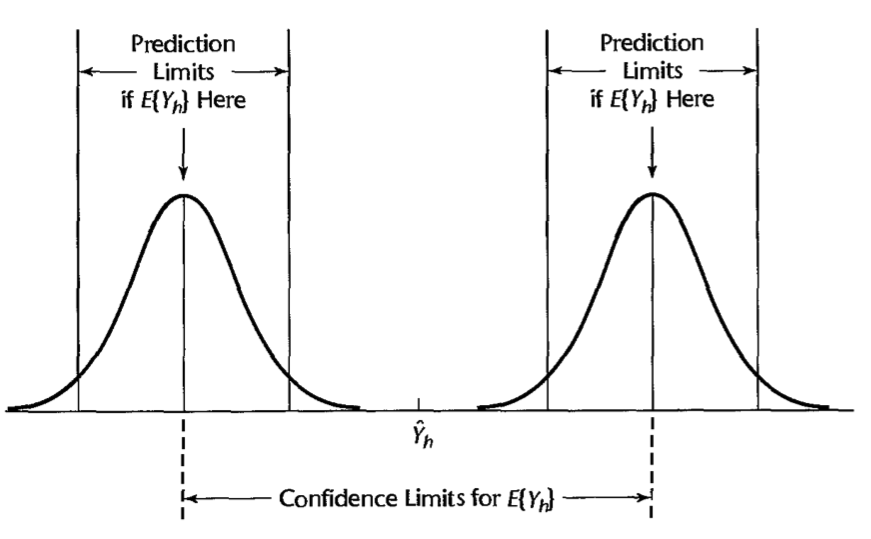
\includegraphics[width=\textwidth/2]{prediction_interval_conf_lim}  \\
    However, we cannot substitute these estimate into the previous distribution because $\E(y^*)$ is a random variable. Since we do not know the mean $\E(y^*)$, and only estiamte it by a confidence interval (shown previously), we cannot be certain of the distribution of $Y$. It could be anywhere along within its confidence intervals (for $\E\{Y_h\}$). Hence \textbf{prediction limit} for $y^*_{new}$ must take into account two elements
    \begin{enumerate}
        \item variation in possible location of distribution of $Y$ (i.e. sampling distributino of $\hat{y}^*$)
        \item variation within the probability distribution of $Y$ (namely $\sigma^2$, same as that of error terms')
    \end{enumerate}
    We can prove that
    \[
        \E(y^*_{new} - \hat{y}^*) 
        = \E(y_{new} - \hat{y}|X = x^*)
        = \E(\hat{\beta}_0 + \hat{\beta}_1 x^*) - \E(\hat{y}^*) 
        = 0
    \]
    \[
        Var(y^*_{new} - \hat{y}^*) 
        = Var(\hat{\beta}_0 + \hat{\beta}_1 x^*) + Var(\hat{y}^*)
        = \sigma^2 + \sigma^2 \left[ \frac{1}{n} + \frac{(x^* - \overline{x})^2}{S_{XX}} \right]
        = \sigma^2 \left[ 1+ \frac{1}{n} +\frac{(x^* - \overline{x})^2}{S_{XX}} \right]
    \]
    Note $Cov(y^*_{new}, \hat{y}^*) = 0$ by independence
    \[
        y^*_{new} - \hat{y}^* \, \sim \, \norm(0, \sigma^2 \left[ 1+ \frac{1}{n} +\frac{(x^* - \overline{x})^2}{S_{XX}} \right])
    \]
    An unbiased estimtor of the variance is given by 
    \[
        s^2(y^*_{new} - \hat{y}^*) = MSE \left[ 1+ \frac{1}{n} +\frac{(x^* - \overline{x})^2}{S_{XX}} \right]
    \]
    \textbf{Standardization of $y^*_{new}$} gives 
    \[
        T = \frac{y^*_{new} - \hat{y}^*}{s^2(y^*_{new} - \hat{y}^*)} \, \sim \, t_{n-2}
    \]
    The $(100-\alpha)\%$ \textbf{Prediction limit} for $y^*_{new}$ at $X=x^*$ is thus given by,
    \[
        (\hat{\beta}_0 + \hat{\beta}_1 x^*) \, \pm \, t_{1-\alpha/2, n-2} MSE \sqrt{1+ \frac{1}{n} +\frac{(x^* - \overline{x})^2}{S_{XX}} } 
    \]
\end{defn*}

\begin{defn*}
    \textbf{Comments}
    \begin{enumerate}
        \item prediction limit is subject to departure from normality of error term distributions
        \item A confidence interval represents an inference on a paramter and is an interval that is intended to cover the value of \textbf{parameter}. A prediction interval, is a statement about the value to be taken by a \textbf{random variable}, the new observation $y^*_{new}$
    \end{enumerate}
\end{defn*}
 

\subsection*{Confidence-band for Regression line} 

\begin{defn*}
    \textbf{Confidence-band} represents uncertainty in the estimate of regression line (i.e. $\E(Y) = \beta_0 + \beta_1 X$)
    
\end{defn*}

\end{document}
